% !TEX root = ../thesis.tex

%%%%%%%%%%%%%%%%%%%%%%%%%%%%%%%%%%%%%%%%%%%%%%%%%%%%%%%%%%%
% Chapter: Background
%%%%%%%%%%%%%%%%%%%%%%%%%%%%%%%%%%%%%%%%%%%%%%%%%%%%%%%%%%%
\chapter{Background}\label{Background}

%%%%%%%%%%%%%%%%%%%%%%%%%%%%%%%%%%%%%%%%%%%%%%%%%%%%%%%%%%%
% Section: CCC
%%%%%%%%%%%%%%%%%%%%%%%%%%%%%%%%%%%%%%%%%%%%%%%%%%%%%%%%%%%
\section{Cross Cutting Concerns}\label{Cross Cutting Concerns}
There is significant research in software engineering that focuses on the importance of software modularity. 
The most significant, among the many, advantage of modular systems is the extensibility and evolution of a system \cite{parnas1972criteria}.

However, during the development of a system there is a number of concerns that have to be considered and implemented into the system. 
In order to follow the modularity principles, those concerns have to be implemented in separate modules, this way the program will be extensible and its evolution will be easier.
Nonetheless, many of those concerns can not fit into the existing modular mechanisms in any of the existing programming paradigms including both \ac{oop} and \ac{pp} \cite{kiczales1997aspect}. 
In those cases, the concerns are scattered through the modules of the system, resulting to scattered and tangled code. 
Those concerns are called \acrlong{ccc} \cite{hannemann2005role}.
\ac{ccc} are considered a serious issue for the evolution of a system and their effects of tangled and scattered code can be disastrous for a system's extensibility.

The reason is that the code which is related to a concern is scattered in multiple modules, while the concern code is tangled with the each module's logic resulting in a system, which does not follow the \textit{Single Responsibility Principle} and consequently is hard to maintain and evolve.

Among many examples of those \ac{ccc} are persistence, caching, logging, error handling \cite{lippert2000study} and access control. 
Additionally, some design patterns scatter ``design pattern code'' through the application, for instance the \textit{Observer Pattern}, \textit{Template Pattern}, \textit{Command Pattern} etc. \cite{hannemann2002design} \cite{marin2004refactoring}.

In order to solve this problem we need a way to refactor and transform the non-modularized \ac{ccc} into a modular \textit{aspect}.
In other words, refactorings of \ac{ccc} should replace all the scattered and tangled code of a concern with an equivalent module \cite{hannemann2005role}, which in \ac{aop} terminology is called \textit{aspect} \cite{kiczales1997aspect}.

%%%%%%%%%%%%%%%%%%%%%%%%%%%%%%%%%%%%%%%%%%%%%%%%%%%%%%%%%%%%%%%%%%%%%%%%%%%%%%%
% Section: AOP
%%%%%%%%%%%%%%%%%%%%%%%%%%%%%%%%%%%%%%%%%%%%%%%%%%%%%%%%%%%%%%%%%%%%%%%%%%%%%%%
\section{Aspect Oriented Programming}\label{Aspect Oriented Programming}

Kiczales et al. present \ac{aop} \cite{kiczales1997aspect} by using an example of a very simple image processing application. 
In that system, as in every system, whenever two properties that are being programmed must compose different tasks and yet be coordinated (in the example filters and loop-fusion), they \textbf{crosscut} each other.
Because general purposes languages provide only one composition mechanism, which leads to complexity and tangling, the programmer must do the co-composition manually.
According to their theory, a system's property can be either a \textit{component}, if it can be clearly encapsulated in a generalized procedure, or it is an \textit{aspect}, which is the opposite.
\ac{aop} supports the programmer in separating components and aspects from each other, by providing mechanisms that make it possible to abstract and compose them together when producing the whole system, a process called \textit{aspect weaving}.
Alternatively to the common programming paradigms, \ac{oop} and \ac{pp}, that allow programmers to only separate the \textit{components} from each other but crosscut the concerns.

However, implementing \ac{aop} programs is not that easy since several tools are needed in order to succeed. 
More specifically, a general purpose language needs only a language, a \textit{compiler} and a \textit{program} written in the language that implements the application.
In the case of an \ac{aop} based implementation, a program consists of a \textit{component language}, in which the components are programmed, one or more \textit{aspect languages}, in which the aspects are programmed, an aspect \textit{weaver} for the combined languages, a \textit{component program} that implements the components using the component language and finally, one or more \textit{aspect programs} that implement the aspects using the aspect languages.
Additionally, an essential function of the aspect weaver is the concept of \textit{join points}, namely the elements of the component language semantics that the aspect programs coordinate with. 

%%%%%%%%%%%%%%%%%%%%%%%%%%%%%%%%%%%%%%%%%%%%%%%%%%%%%%%%%%%%%%%%%%%%%%%%%%%%%%%
\subsection{AspectJ}\label{AspectJ}
There is significant work in the area of aspect oriented languages but one the most important contribution is the AspectJ\footnote{\url{https://eclipse.org/aspectj/}} project, which is a simple and practical aspect-oriented extension to Java and it has been introduced by Kiczales et al. \cite{kiczales2001overview}.
The authors of AspectJ provide examples of programs developed in AspectJ and show that by using it, \ac{ccc} can be implemented in clear form, which in other general purpose languages would lead to tangled and scattered code. 
AspectJ was developed as a compatible extension to Java so that it would facilitate adoption by current Java programmers. 
The compatibility lays on upward compatibility, platform compatibility, tool compatibility and programmer compatibility. One of the most important characteristics of AspectJ is that it is not a \ac{dsl} but a general purpose language that uses Java's static type system.
Our goal is to apply those properties for our managed data implementation.

%%%%%%%%%%%%%%%%%%%%%%%%%%%%%%%%%%%%%%%%%%%%%%%%%%%%%%%%%%%%%%%%%%%%%%%%%%%%%%%
\subsection{Design Patterns in Aspect Oriented Programming}\label{Design Patterns in Aspect Oriented Programming}

Hannemann et al. present a showcase of \ac{aop} \cite{hannemann2002design} in which they conduct an aspect-oriented implementation of the Gang of Four design patterns \cite{gamma1995design} in AspectJ, in which 17 out of 23 cases show modularity improvements.
Even though design patterns offer flexible solutions to common software problems, those patterns involve crosscutting structures between roles and classes / objects. 
There are several problems that the \ac{oop} design patterns introduce in respect to \ac{ccc}, specifically in cases when one object plays multiple roles, many objects play one role, or an object play roles in multiple patterns \cite{sullivan2002advanced} (design pattern composition).

The problem lays on the way a design pattern influences the structure of the system and its implementation. 
Pattern implementations are often binded to the instance of use resulting in their scattering into the code and losing their modularity \cite{hannemann2002design}.

Even worse, in case of multiple patterns used in a system (pattern overlay and pattern composition), it can become difficult to trace particular instances of a design pattern. 
Composition creates large clusters of mutually dependent classes\cite{sullivan2002advanced} and some design patterns explicitly use other patterns in their solution.

% \subsubsection{Observer pattern in Aspect Oriented Programming}\label{Observer pattern in Aspect Oriented Programming}
% Hannemann et al. \cite{hannemann2002design} provide some example implementations of several design patterns, including the \textit{Observer Pattern} in which they focus on a detailed implementation.
% As they mention, in an observer pattern implementation, both the \textit{Subject} and the \textit{Observer} have to know about their roles and have ``pattern related code'' in them. 
% As a result, adding or removing code from a class requires changes of code in that class. 

% In their implementation \cite{hannemann2002design} of the observer pattern in AspectJ, they separate abstract aspects for: 

% \begin{itemize}
% 	\item The \textit{Subject} and \textit{Observer} roles in classes.

% 	\item Maintenance of a mapping from \textit{Subjects} to \textit{Observers}.

% 	\item The trigger of \textit{Subjects} that update \textit{Observers}.
% \end{itemize}

% And concrete aspects for each instance of the pattern fills in the specific parts:
% \begin{itemize}
% 	\item Which classes can be \textit{Subjects} and which \textit{Observers}.

% 	\item A set of changes on the \textit{Subjects} that triggers the \textit{Observers}.

% 	\item The specific means of updating each kind of \textit{Observer} when the update logic requires it.
% \end{itemize}

\subsubsection{Modularity Properties}\label{BG Modularity Properties}
Hannemann et al. \cite{hannemann2002design} provide some example implementations of several design patterns.
During the assessment of their findings, the authors used four \textit{modularity properties}.
In this thesis we used the same properties to assess our refactoring in relation to the \ac{aop} version.
The modularity properties are the following:

\begin{description}
	\item [Locality]
	The \textit{locality} property refers to the ability of an existing class to be incorporated into a pattern instance with effortless adaptation. 
	In this case, all the changes have to be made in the pattern instance.

	\item [Reusability]
	\textit{Reusability} holds when a class is not coupled to its role in a pattern.
	Therefore, it can be used in different contexts without modifications and the reusability of participants can be increased.

	\item [(Un)pluggability]
	Both the \textit{locality} and the \textit{reusability} properties of a system make the pattern implementations \textit{(un)pluggable}.

	\item [Composition transparency]
	Having achieved \textit{locality} and \textit{reusability}, we have obtained an \textit{(un)pluggable} system.
	This suggests that we can reuse generalized pattern code and localize the code for a particular pattern instance.
	Thus, creating multiple instances of the same pattern in one application, it is easier to understand (\textit{composition transparency}).
	This way the problem of having multiple instances of a design pattern in one application is solved.
\end{description}

%%%%%%%%%%%%%%%%%%%%%%%%%%%%%%%%%%%%%%%%%%%%%%%%%%%%%%%%%%%%%%%%%%%%%%%%%%%%%%%
\subsection{Evolvability issues}\label{Aspect Oriented Programming Evolvability}
Since modularization and separation of concerns make the evolution of an application a lot easier and \ac{aop} provides mechanisms for modularization and system decomposition, aspect-oriented programs should be easier to be evolved and maintained.
Paradoxically, this is not the case since \ac{aop} technologies deliver applications that are as hard, and sometimes even harder, as non-\ac{aop}.

According to Tourwe et al. \cite{tourwe2003existence} the problem is that aspects have to include a crosscut description of all places in the application.
Thus, it is much harder to make such crosscuts oblivious to the application and most importantly to the rest of the modules. 
Additionally, current means for specifying concerns rely heavily in the existing structure of the application, therefore the aspects are tightly coupled to the application (and its structure) and consequently this affects negatively the evolvability of a system since it makes it hard to change its structural.
As Tourwe et al. propose, a solution for this problem would be the creation of a new, more sophisticated crosscut language. 
A language that enables the developer to discriminate between methods based on what they actually do instead of what they look like, in a more intentional way.
This new language that implements aspects in a modular way is something try to realize in our thesis.

%%%%%%%%%%%%%%%%%%%%%%%%%%%%%%%%%%%%%%%%%%%%%%%%%%%%%%%%%%%%%%%%%%%%%%%%%%%%%%%
% Section: Managed Data 
%%%%%%%%%%%%%%%%%%%%%%%%%%%%%%%%%%%%%%%%%%%%%%%%%%%%%%%%%%%%%%%%%%%%%%%%%%%%%%%
\section{Managed Data}\label{Managed Data}
Managed data \cite{loh2012managed} is a data abstraction mechanism that allows the programmer to control the definition of the data and their manipulation mechanisms. 
Additionally it provides a modular way to control aspects of data.
Managed data helps the programmer by giving them control over the structuring mechanisms, which until now were predefined by the programming languages. 
The developers could not take control of them, they could only create data of those types.
Managed data provides significant flexibility since it lifts data management up to the application level, by allowing the programmer to build data managers that handle the fundamental data manipulation primitives, normally hard-coded into the programming language. 

Managed data has three essential components:

\begin{description}
	\item [Data description language,] that describes the desired structure and properties of data.

	\item [Data managers,] that enable creation and manipulation of instances of data.

	\item [Integration,] with a programming language to allow data to be created and manipulated.
\end{description}

In the traditional approach, the programming language includes data definition mechanisms and their processes, which are both predefined. 
However, with managed data, the data structuring mechanisms are defined by the programmer by interpretation of data definitions.
Of course, since a data definition model is also data, it requires a meta-definition mechanism.

%%%%%%%%%%%%%%%%%%%%%%%%%%%%%%%%%%%%%%%%%%%%%%%%%%%%%%%%%%%%%%%%%%%%%%%%%%%%%%%
\subsection{Schemas}\label{Schemas}
The schemas are the way to describe the structure of the data to be managed. 
They can be just a simple data description language which programmers can use to describe simple kind of data. 
For example Cook et al. \cite{loh2012managed} used Ruby hash for the data description on a simple example where the hash was an object that represented a mapping from values to values. 
However, a simple schema format like this can not be used to describe itself because it is not a record. 
Therefore, we need a more descriptive language that defines records and fields of records.

% A self-describing schema would allow schemas to be managed data themselves. 
% We therefore need a self-describing schema that can be used to describe schemas, namely the ``Schema-Schema''. 
% A Schema-Schema is also managed data with its own data manager.
% This process is called \textit{Bootstrapping} and it is needed in order to ``jumpstart'' the process. 
% This extends the benefits of programmable data structuring to their own implementation.
% Schemas can be interpreted in many different ways to create different kinds of records based on the manipulation provided by the data managers.

%%%%%%%%%%%%%%%%%%%%%%%%%%%%%%%%%%%%%%%%%%%%%%%%%%%%%%%%%%%%%%%%%%%%%%%%%%%%%%%
\subsection{Data Managers}\label{Data Managers}
Data managers are the mechanisms that interpret \textit{schemas} with defined manipulation strategies set by the programmers. 
The input to a data manager is a schema, which describes the structure of the data to be managed.
Since the schema is only known dynamically, the data managers must be able to determine the fields of the managed data object dynamically as well.
In order to implement such an operation we need a meta-programming mechanism that dynamically analyses the structure of a schema and applies to it the functionality of the data managers.
In their implementation Cook et al. \cite{loh2012managed} used the ``missing\_method'' implementation in order to succeed that.
In our case we will use the reflection API and dynamic proxies.

%%%%%%%%%%%%%%%%%%%%%%%%%%%%%%%%%%%%%%%%%%%%%%%%%%%%%%%%%%%%%%%%%%%%%%%%%%%%%%%
% Section: Reflection
%%%%%%%%%%%%%%%%%%%%%%%%%%%%%%%%%%%%%%%%%%%%%%%%%%%%%%%%%%%%%%%%%%%%%%%%%%%%%%%
\section{Java Reflection and Dynamic Proxies}\label{Java Reflection and Dynamic Proxies}
The Java programming language provides the programmer with a Reflection API\footnote{\url{https://docs.oracle.com/javase/tutorial/reflect/}} that offers the ability to examine or modify the runtime behavior of applications running in the \ac{jvm}. 
Additionally, Java comes with an implementation of Dynamic Proxies\footnote{\url{https://docs.oracle.com/javase/8/docs/api/java/lang/reflect/Proxy.html}} which is a class that implements a list of interfaces specified at runtime.

%%%%%%%%%%%%%%%%%%%%%%%%%%%%%%%%%%%%%%%%%%%%%%%%%%%%%%%%%%%%%%%%%%%%%%%%%%%%%%%
\subsection{Reflection}\label{Reflection}

Reflection is the ability of a running program to examine itself and its environment and to change what it does depending on what it finds \cite{forman2004java}.

In order for this self-examination to be successful, the program needs to have a representation of itself as \textit{metadata}.
In a \ac{oop} language this metadata are organized into objects, hence they are called \textit{metaobjects}. 
Finally, the process of the runtime self-examination of these metaobjects is called \textit{introspection}.

Java supports reflection through its reflection API since the version 1.1.
Using Java reflection a running program can learn a lot about itself. 
This information may derive from classes (the \texttt{Class} metaobject), class name, class methods, a class super and sub classes, methods (the \texttt{Method} metaobject), method name, method parameters, method type, variables, variables handlers and more. 
Querying information from these metaobjects is called introspection.
Additionally to the examining of the these metaobjects, a developer has the ability to dynamically call a method that is discovered at runtime. 
This process is called \textit{dynamic invocation}. 
Using dynamic invocation, a \texttt{Method} metaobject can be instructed to invoke the method that it represents during the program's runtime. 

Although reflection is considered helpful for developing flexible software, it has some known pitfalls:

\begin{description}
	
	\item[Security.] Since metaobjects give a developer the ability to invoke and change underlined data of the program, it also gives access them to places that are supposed to be secure (e.g. \texttt{private} variables).

	\item[Code complexity.] Consider a program that uses both normal objects and metaobjects. 
	That introduces an extra level of complexity since now a developer has to deal with different kinds of objects on different levels, meta and normal level.

	\item[Runtime performance.] Of course the runtime dynamic examination and introspection introduce significant overhead on most language implementations. 
	In the case of Java's dynamic proxies a 6.5x overhead observed \cite{marr2015zero}. 
	However, this is not something that we take into consideration in our implementation.

\end{description}

%%%%%%%%%%%%%%%%%%%%%%%%%%%%%%%%%%%%%%%%%%%%%%%%%%%%%%%%%%%%%%%%%%%%%%%%%%%%%%%
\subsection{Dynamic Proxies}\label{Dynamic Proxies}
Since 1.3 version Java supports the concept of \textit{Dynamic Proxies}.
A \textit{proxy} is an object that supports the interface of another object (\textit{target}), so that the proxy can substitute for the target for all practical purposes \cite{forman2004java}.
A proxy has to have the same interface as the \textit{target} so that it can be used in exactly the same way. 
Additionally it \textit{delegates} some or all of the calls that it receives to its target and thus acts as either an intermediary or a substitute object.
As a result, a programmer has the capability to add behavior to objects dynamically. 
The Java reflection API contains a dynamic proxy-creation facility, in \texttt{java.lang.reflect.Proxy}.

There are several examples of dynamic proxies implementation in Java including implicit conformance, future invocations \cite{pratikakis2004transparent}, dynamic multi dispatch, design by contract or \ac{aop} \cite{eugster2006uniform}.

\subsubsection{Proxy Objects}\label{Proxy Objects}
A proxy is an object which conforms to a set of interfaces, for which that proxy was created for. 
The corresponding proxy class extends the class \texttt{Proxy} and implements all its interfaces.
Thus, conforming to all those interfaces, a proxy can be casted to any of them and any method defined in those interfaces can be invoked on the proxy object \cite{eugster2006uniform}.

\subsubsection{Invocation Handlers}\label{Invocation Handlers}
All the proxy objects have an associated object of type \texttt{InvocationHandler}, which handles the method invocations performed on the proxy. 
Its interface is shown in Listing \ref{lst:The Invocation Handler Interface}.

\begin{sourcecode}
	\begin{lstlisting}[language=Java]
public interface InvocationHandler {
	public Object invoke(Object proxy, Method method,Object[] args) throws Throwable;
}		
	\end{lstlisting}
	\caption{The Invocation Handler Interface}
	\label{lst:The Invocation Handler Interface}
\end{sourcecode}

The arguments of the \texttt{invoke} method include the object on which the method was originally invoked (i.e., the proxy), the method itself that was invoked on the proxy, and the arguments of that method, if any.
Therefore, the \texttt{invoke} method is capable of handling any method invocation.

\subsubsection{Issues}\label{Dynamic Proxies Issues}
A proxy instance is an object and it responds to the methods declared by \texttt{java.lang.Object}. 
Thus, when these methods should be invoked and from which object is an issue that arises \cite{forman2004java}.

The methods \texttt{equals}, \texttt{hashCode}, and \texttt{toString} are inherited by all classes from the \texttt{Object} class and they are handled just like custom methods.
If they are proxied then they are also overridden by the proxy classes and invocations to them are forwarded to the invocation handler of the proxy. 
Other methods defined in \texttt{Object} are not overridden by proxy classes, as they are \texttt{final} \cite{eugster2006uniform}.

% \subsubsection{Logging Example}
% Previously, Section \ref{Cross Cutting Concerns}, we mentioned the \textit{logging} \ac{ccc}.
% Imagine that every method invocation of an object has to be logged into the console, in that case we would need to write logging code on each of the methods of that class.
% This would lead to scattered logging code through the methods.
% This is problem can be solved with dynamic proxies and a simple solution is presented in Listing \ref{lst:Logging in dynamic proxies}.

% \begin{sourcecode}[H]
% 	\begin{lstlisting}[language=Java]
% public class TracingIH implements InvocationHandler {
	
% 	public static Object createProxy(Object obj, PrintWriter out) {
% 		return Proxy.newProxyInstance(
% 			obj.getClass().getClassLoader(), 
% 			obj.getClass().getInterfaces(), 
% 			new TracingIH( obj, out));
% 	}

% 	private Object target;
% 	private PrintWriter out;

% 	private TracingIH(Object obj, PrintWriter out) {
% 		target = obj;
% 		this.out = out;
% 	}

% 	public Object invoke(Object proxy, Method method,Object[] args) throws Throwable {
% 		Object result = null;

% 		try {
% 			out.println(method.getName() + "(...) called" );
% 			result = method.invoke( target, args );
% 		} catch (InvocationTargetException e) {
% 			out.println(method.getName() + " throws " + e.getCause());
% 			throw e.getCause();
% 		}
% 		out.println(method.getName() + " returns" );
% 		return result;
% 	}
% }
% 	\end{lstlisting}
% 	\caption{An invocation handler for a proxy that traces calls \cite{forman2004java}}
% 	\label{lst:Logging in dynamic proxies}
% \end{sourcecode}

%%%%%%%%%%%%%%%%%%%%%%%%%%%%%%%%%%%%%%%%%%%%%%%%%%%%%%%%%%%%%%%%%%%%%%%%%%%%%%%
% Section: JHotDraw
%%%%%%%%%%%%%%%%%%%%%%%%%%%%%%%%%%%%%%%%%%%%%%%%%%%%%%%%%%%%%%%%%%%%%%%%%%%%%%%
\section{JHotDraw And AJHotDraw}\label{JHotDraw And AJHotDraw}
JHotDraw\footnote{\url{http://www.jhotdraw.org/}} is a Java GUI framework for technical and structured graphics. 
It is an open-source, well-designed and flexible drawing framework of around 18,000 non-comment lines of Java code. 
JHotDraw's  design relies heavily on some well-known design patterns \cite{gamma1995design} and it is considered as a showcase for software quality techniques provided to the \ac{oop} community. 

The fact that JHotDraw is praised for its design makes it an ideal candidate as a showcase for an aspect oriented migration. 
Marin and Moonen \cite{marinajhotdraw} use this showcase for adoption of aspect-oriented techniques in existing systems. 
In particular, they present AJHotDraw\footnote{\url{http://swerl.tudelft.nl/bin/view/AMR/AJHotDraw}}, which is an aspect-oriented version of JHotDraw developed in Java and AspectJ. 
The goal of AJHotDraw is to take JHotDraw and migrate it to a functionally equivalent aspect-oriented version. 

The authors presented a fan-in analysis of JHotDraw \cite{marin2004identifying} and implemented an idiom-driven approach to aspect-mining. 
This way they could extract a number of aspects in JHotDraw. 
Next, they performed a concern exploration in order to expand their mining results, leading to concern sorts.
Concern sorts is a consistent way to address crosscutting concerns in source code \cite{marin2005classification}.
This led to the identification and documentation of \ac{ccc} in JHotDraw, which helps the developers to identify \ac{ccc} in it.
In order to handle the aspects in a more consistent and formal way, Marin et al. provided a list of \textit{template aspect} solutions for their concern sorts.
Finally, they performed aspect refactoring of JHotDraw by presenting the AJHotDraw, which according to them, was the largest migration to aspects available to date.
Their refactoring aimed at maintaining the conceptual integrity of the original design.

In order to refactor the existing framework, the first thing that AJHotDraw developers needed to do was to create a test subproject for the JHotDraw, called TestJHotDraw\footnote{\url{http://swerl.tudelft.nl/bin/view/AMR/TestJHotDraw}}, which ensures behavioral equivalence between the original and the refactored solution. 
Refactoring implies preserving the observable behavior of an application \cite{fowler2009refactoring} and since the developers of AJHotDraw ought to test their functionality, TestJHotDraw was created. 
There are several contributions of the aspect-oriented implementation approach \cite{marinajhotdraw}. 
The authors suggest that the project contributes to a gradual and safe adoption of aspect-oriented techniques in existing applications and allows for a better assessment of aspect orientation.

In this thesis we have used JHotDraw and AJHotDraw in order to evaluate our aspect refactoring in managed data.
However, TestJHotDraw is written in AspectJ, a language we did not want include in our project, and therefore it is not used.
Instead, we used the JHotDraw original test suite, which consists of 1218 test cases, for our refactoring behavioral preservation.
The aspect refactoring process is described in Chapter \ref{AspectRefactoring}.

%%%%%%%%%%%%%%%%%%%%%%%%%%%%%%%%%%%%%%%%%%%%%%%%%%%%%%%%%%%%%%%%%%%%%%%%%%%%%%%
\subsection{Refactoring of Crosscutting Concerns}\label{Refactoring of ccc}
The refactoring of legacy code to aspect oriented code is also known as \textit{Aspect Refactoring} \cite{marin2005approach}. 
During this process it is important to identify which elements are going to be refactored and which \textit{aspect} solutions will replace them. 
To evaluate the refactored elements \cite{fowler2009refactoring}, a testing component is needed in order to ensure behavior conservation, hence some coherent criteria to organize \ac{ccc} are needed. 
Marin, Moonen and Deursen \cite{marin2005approach} organize the \ac{ccc} into types, which are descriptions of similar concerns that share the following properties: 

\begin{itemize}
	\item A generic behavioral, design or policy requirement to describe the concern within a formalized, consistent context (e.g., role superimposition to modular units (classes), enforced consistent behavior, etc.),

	\item An associated legacy implementation idiom in a given (non-aspect oriented) language (e.g., interface implementations, method calls, etc.)

	\item An associated (desired) aspect language mechanism to support the modularization of the type's concerns (e.g., \texttt{pointcut} and \texttt{advice}, introduction, composition models).
\end{itemize}

%%%%%%%%%%%%%%%%%%%%%%%%%%%%%%%%%%%%%%%%%%%%%%%%%%%%%%%%%%%%%%%%%%%%%%%%%%%%%%%
\subsection{The Observer Pattern}\label{The Observer Pattern}
As discussed, design patterns introduce \ac{ccc} by scattering ``pattern code'' through an application.
Hannemann et al. \cite{hannemann2005role} discuss this with an example of \ac{ccc} refactoring of the observer pattern.
% The observer pattern is by nature not-modularized. 
% The pattern crosscuts a large number of modules, tangling the scattered concern implementation with the component code and complicating changes.

\subsubsection{Role-based Refactoring}
The authors present a \textit{role-based} refactoring, which consists of classifying the roles of the pattern in different aspects.
The role-based refactoring approach helps the developer to transform a scattered implementation of \ac{ccc} into an equivalent but modular \ac{aop} implementation. 
Both \ac{ccc} and refactoring are described in terms of roles. 

According to the authors \cite{hannemann2005role}, the steps of role-based refactoring are the following:
\begin{description}

	\item [Selecting a \ac{ccc} refactoring:] The refactoring includes an abstract description of the \ac{ccc} it targets and a set of instructions to produce a modular AOP implementation of the refactoring (e.g. the Observer pattern \ac{ccc} refactoring).

	\item [Stating a mapping:] Map role elements comprising the \ac{ccc} description to the program elements of the scattered code (e.g. the Subject and the Observer role to concrete classes)

	\item [Planning the refactoring:] make the right choices for specific cases since a \ac{ccc} refactoring involves modifying several parts of a codebase (e.g. naming).

	\item [Execution:] transform the code according to the refactoring instructions (e.g. modularizes Observer pattern as a result).
\end{description}

Thus, to refactor \ac{ccc} it is required a mapping from the abstract \ac{ccc} description to programming components that explicitly describe the \ac{ccc} implementation.
% This mapping for the case of the observer pattern is presented in Figure \ref{fig:Observer_Role_Mapping}.

% \begin{figure}[H]
% 	\centering
%   	\fbox{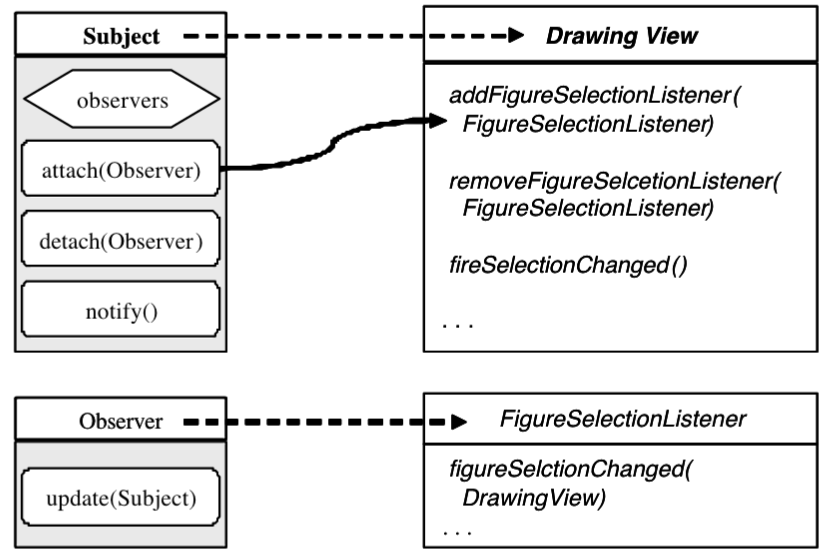
\includegraphics[width=.50\textwidth]{figures/observer_pattern_role_mapping.png}}
%   	\caption{Observer pattern: Role Mapping \cite{hannemann2005role}}
%   	\label{fig:Observer_Role_Mapping}
% \end{figure}

% This figure describes the roles mapping in a specific case on JHotDraw, the \textit{Figure Selection Listener}.
% However the authors have shown an abstract and reusable way of describing those roles.

%%%%%%%%%%%%%%%%%%%%%%%%%%%%%%%%%%%%%%%%%%%%%%%%%%%%%%%%%%%%%%%%%%%%%%%%%%%%%%%
\subsection{The Figure Selection Observer of JHotDraw}\label{The Figure Selection Observer of JHotDraw}
% As mentioned above, Hannemann et al. \cite{hannemann2005role} presented a refactoring of the \textit{Observer} design pattern in JHotDraw.
During the AJHotDraw implementation\cite{marin2005approach}, the authors proposed a type-based refactoring on the same \textit{Observer} instance, as Hannemann did \cite{hannemann2005role}, the \texttt{FigureSelectionListener}.

The concern sorts identified in this case are: the \textit{Role Superimposition}, which is similar to the role-based refactoring described previously and the \textit{Consistent Behavior}, which describes a set of methods consistently invoking a specific action as a step in their execution.

The legacy design of JHotDraw is displayed in Figure \ref{fig:Selection_Listener}.

\begin{figure}[H]
	\centering
  	\fbox{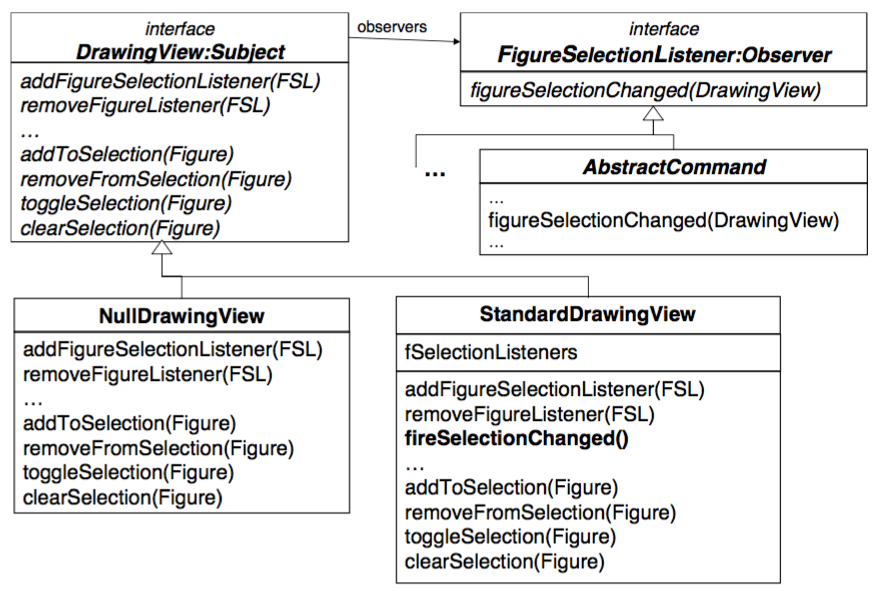
\includegraphics[width=.5\textwidth]{figures/BG_Observer_pattern_Selection_Listener.png}}
  	\caption{Observer pattern: Selection Listener \cite{marin2005approach}}
  	\label{fig:Selection_Listener}
\end{figure}

The \texttt{FigureSelectionListener} has the \textit{Observer} role in the pattern implementation. 
Any class that is subject to changes of the selection of figures in a \texttt{DrawingView}, implements this interface. 
The \texttt{DrawingView} interface partially defines the \textit{Subject} role by including two methods \texttt{addViewChangeListener} and \texttt{removeViewChangeListener}.
From the classes that implement this interface only one, the \texttt{StandardDrawingView}, contains a non-empty implementation of the \textit{Subject} role in the \texttt{fireSelectionChanged} method.
Note that this method is only defined in the concrete class, which deviates from the standard Observer pattern implementation.

In their aspect refactoring, they described an aspect that is constructed comprising both the \textit{Subject} and \textit{Observer} roles definition and maintaining a list of associations between each \textit{Subject} and its \textit{Observer} objects.
Their type-based refactoring\cite{marin2005approach} distinguishes several crosscutting elements in JHotDraw's \textit{Observer} pattern. 
First, the role superimposition, applied twice, for each of the two roles. 
Second, consistent behavior to notify the observers of the changes in the \textit{Subject} object.
Where superimposition is defined as the aspect implementation of a specific role and consistent behavior as the aspect implementation of a \textit{consistent behavior} for a number of method elements that can be captured by a natural pointcut.
The \texttt{GenericRole} (empty) interface documents the crosscutting type of role superimposition. 
Specific roles, like \textit{Observer} and \textit{Subject} (\texttt{SelectionSubject}) extend the interface.
These elements are shown in Figure \ref{fig:Concerns_Selection_Listener}.

\begin{figure}[H]
	\centering
  	\fbox{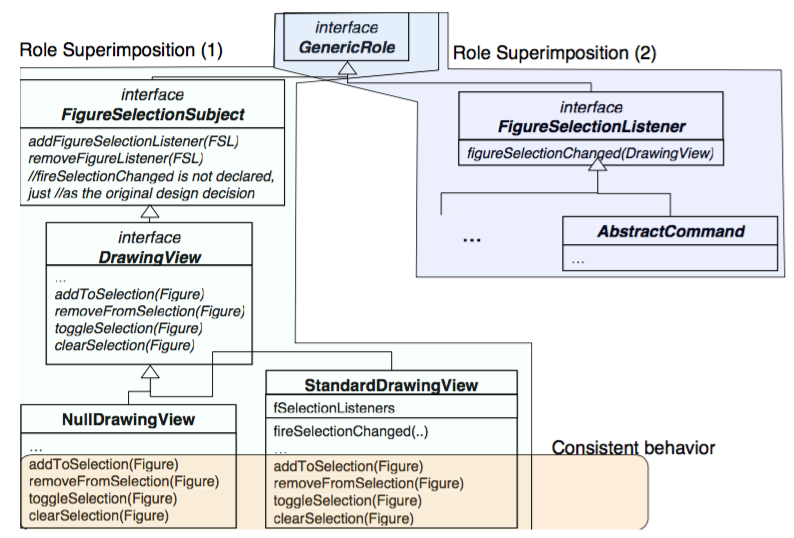
\includegraphics[width=.5\textwidth]{figures/BG_The_concern_types_in_Selection_Listener.png}}
  	\caption{AJHotDraw: The concern types in Selection Listener \cite{marin2005approach}}
  	\label{fig:Concerns_Selection_Listener}
\end{figure}

%%%%%%%%%%%%%%%%%%%%%%%%%%%%%%%%%%%%%%%%%%%%%%%%%%%%%%%%%%%%%%%%%%%%%%%%%%%%%%%%
\subsection{The ``Undo'' Concern of JHotDraw}\label{The Undo Concern of JHotDraw}
Marin et al. have also identified the  ``Undo'' concern in JHotDraw. 
A number of activities use this functionality including font sizes and colors, image rotation and a lot more.
The authors propose the refactoring of the undo concern and more specifically a specific case the \textit{Change Attribute Command} \cite{marin2004refactoring}.

A general representation of the elements in the JHotDraw implementation of the ``Undo'' concern can be seen in Figure \ref{fig:Participants_for_undo_in_JHotDraw}.

\begin{figure}[H]
	\centering
  	\fbox{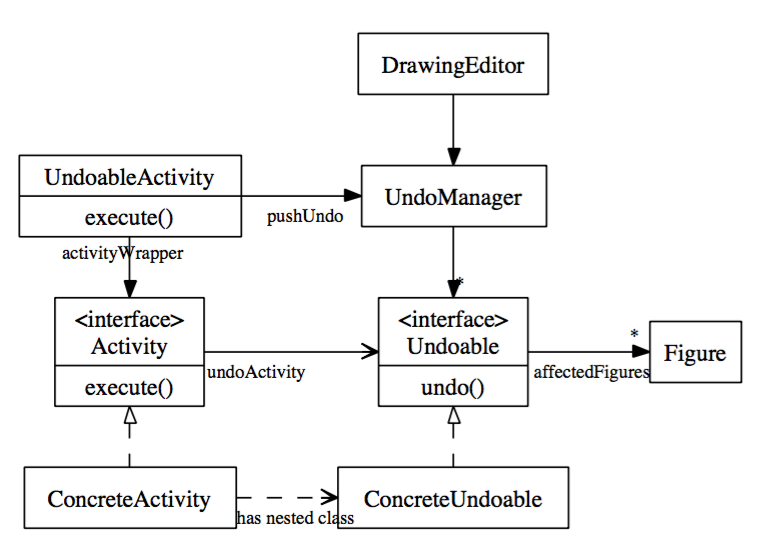
\includegraphics[width=.55\textwidth]{figures/BG_Participants_for_undo_in_JHOTDRAW.png}}
  	\caption{Participants for undo in JHotDraw \cite{marin2004refactoring}}
  	\label{fig:Participants_for_undo_in_JHotDraw}
\end{figure}

The \texttt{Activity} component participates in the implementation of the \textit{Command} design pattern\cite{gamma1995design}. 
Many of these activities have support for undo functionality, which in JHotDraw is implemented by means of nested (undo) classes.
The nested class knows how to undo the given activity which maintains a list of affected figures whose state is also affected if the activity would be ``undone''. 
Whenever the activity modifies its state it also updates fields in its associated undo activity to actually perform the undo. 

The implementation of AJHotDraw succeeded in refactoring this concern in JHotDraw through the following steps \cite{marin2004refactoring}:

\begin{enumerate}

	\item An undo-dedicated aspect is associated to each of undo-able command. 
	The aspect will implement the entire undo functionality for the given command, while the undo code is removed from the command class.

 	\item Each aspect will consistently be named by appending \texttt{UndoActivity} to the name of its associated command class to enforce the relation between the two.

	\item Next, the command's nested \texttt{UndoActivity} class moves to the aspect. 
	The factory methods for the undo activities also move to the the aspect, from where are introduced back, into the associated command classes, using inter-type declarations.

	\item Finally, the undo setup is attached to those methods from which was previously removed, namely execute() method, by means of an AspectJ \texttt{advice}.

\end{enumerate}

In particular, this proposition is applied in the \texttt{ChangeAttributeCommand} \cite{marin2004refactoring}.
The undo \ac{ccc} has been identified, then removed from the system, and finally re-added in an aspect-specific manner.

In this thesis we investigated both the \texttt{FigureSelectionListener} and the \texttt{ChangeAttributeCommand} (\textit{Undo}) concerns by refactoring them in a new version of the JHotDraw and compare them to their \ac{aop} counterpart.

%%%%%%%%%%%%%%%%%%%%%%%%%%%%%%%%%%%%%%%%%%%%%%%%%%%%%%%%%%%%%%%%%%%%%%%%%%%%%%%
% Section: Metrics
%%%%%%%%%%%%%%%%%%%%%%%%%%%%%%%%%%%%%%%%%%%%%%%%%%%%%%%%%%%%%%%%%%%%%%%%%%%%%%%
\section{Metrics}\label{Background Metrics}
There is a number of metrics that are used in empirical studies for software assessment. 
However, most of those metrics refer to \ac{oop} systems \cite{chidamber1994metrics} and their basic abstractions such as class, object, methods and attributes.
Since \ac{aop} introduces a new abstraction, the \textit{aspect}, the available metrics can not be applied to \ac{aop}.

Sant'Anna et al. \cite{sant2003reuse} proposed a new framework for assessing reusability and maintainability qualities of \ac{aop} solutions.
Those metrics are based on previous work from Chidamber and Kemerer \cite{chidamber1994metrics} and are an extension for measuring aspects as well.
Their framework focuses on measurement of the \textit{separation of concerns}, the \textit{coupling}, the \textit{cohesion} and the \textit{size} criteria of an application.
The goal of the framework is that software engineers can use it in order to assess design decisions in both \ac{oop} and \ac{aop} systems.
In this thesis we are going to use this framework to assess and discuss the results of ManagedDataJHotDraw in relation to JHotDraw.

The metrics proposed \cite{sant2003reuse} are grouped in four subsections (criteria) based on the attributes they measure:

\paragraph{Separation Of Concerns}refers to the ability to identify, encapsulate and manipulate those parts of software that are relevant to a particular concern \cite{tarr1999n}.
	\begin{itemize}
		\item \ac{cdc}, counts the number of primary components whose main purpose is to contribute to the implementation of a concern.
		This metric counts the degree of concern \textbf{scattering} in the level of components \cite{figueiredo2008maintainability}.

		\item \ac{cdo}, counts the number of primary operations whose main purpose is to assist the implementation of a concern.
		Constructors also are counted as operations.
		This metric counts the degree of concern \textbf{scattering} in the level of methods \cite{figueiredo2008maintainability}.

		\item \ac{cdloc}, counts the number of transition points for each concern through the lines of code.
		To use this metric it is required a \textit{shadowing process} that partitions the code into shadowed areas and non-shadowed areas. 
		The shadowed areas are lines of code that implement a given concern. 
		Transition points are the points in the code where there is a transition from a non-shadowed area to a shadowed area and vice-versa \cite{garcia2003agents}.
		Therefore, the higher the \ac{cdloc}, the more intermingled is the concern code within the implementation of the components; the lower the \ac{cdloc}, the more localized is the concern code.
		This metrics aims to compute the degree of concern \textbf{tangling} \cite{figueiredo2008maintainability}.
	\end{itemize}

\paragraph{Coupling}is an indication of the strength of interconnections between the components in a system. Highly coupled systems have strong interconnections, with program units dependent on each other \cite{sommerville2004software}.
	\begin{itemize}
		\item \ac{cbc}, is defined for a component (class or aspect) as the number of other components to which it is coupled.

		\item \ac{dit}, counts how far down the inheritance hierarchy a class (or aspect) is declared.
	\end{itemize}

\paragraph{Cohesion}of a component is a measure of the closeness of the relationship between its internal components \cite{sommerville2004software}.
	\begin{itemize}
		\item \ac{lcoo}, measures the lack of cohesion of a component.
		The metric is an extension ofChidamber and Kemerer's \cite{chidamber1994metrics} \ac{lcom} metric.
		More specifically, it measures the amount of method / advice pairs which do not access the same instance variable.
	\end{itemize}

\paragraph{Size}measures the length of a software system's design and code.
	\begin{itemize}
		\item \ac{vs}, counts the number of system components.
		Those components are classes, in case of \ac{oop}, or classes and aspects, in case of \ac{aop}.
		The component instances are not counted.

		\item \ac{loc}, counts the number of code lines.
		Documentation, comments and blanks are omitted.

		\item \ac{noa}, counts the internal vocabulary of each component.
		The metric counts the number of fields of each class or aspect.
		Inherited attributes are not included in the count.

		\item \ac{woc}, measures the complexity of a component in terms of its operations.
		This metric extends the Chidamber and Kemerer's \cite{chidamber1994metrics} \ac{wmc} metric for \ac{aop}.
	\end{itemize}

Garcia et al. \cite{garcia2003agents} present an overview of these metrics in terms of the Goal / Question / Metric (GQM) approach \cite{wohlin2012experimentation} \ac{lcom} can be seen in Figure \ref{fig:metrics_questions}.

\begin{figure}[H]
	\centering
  	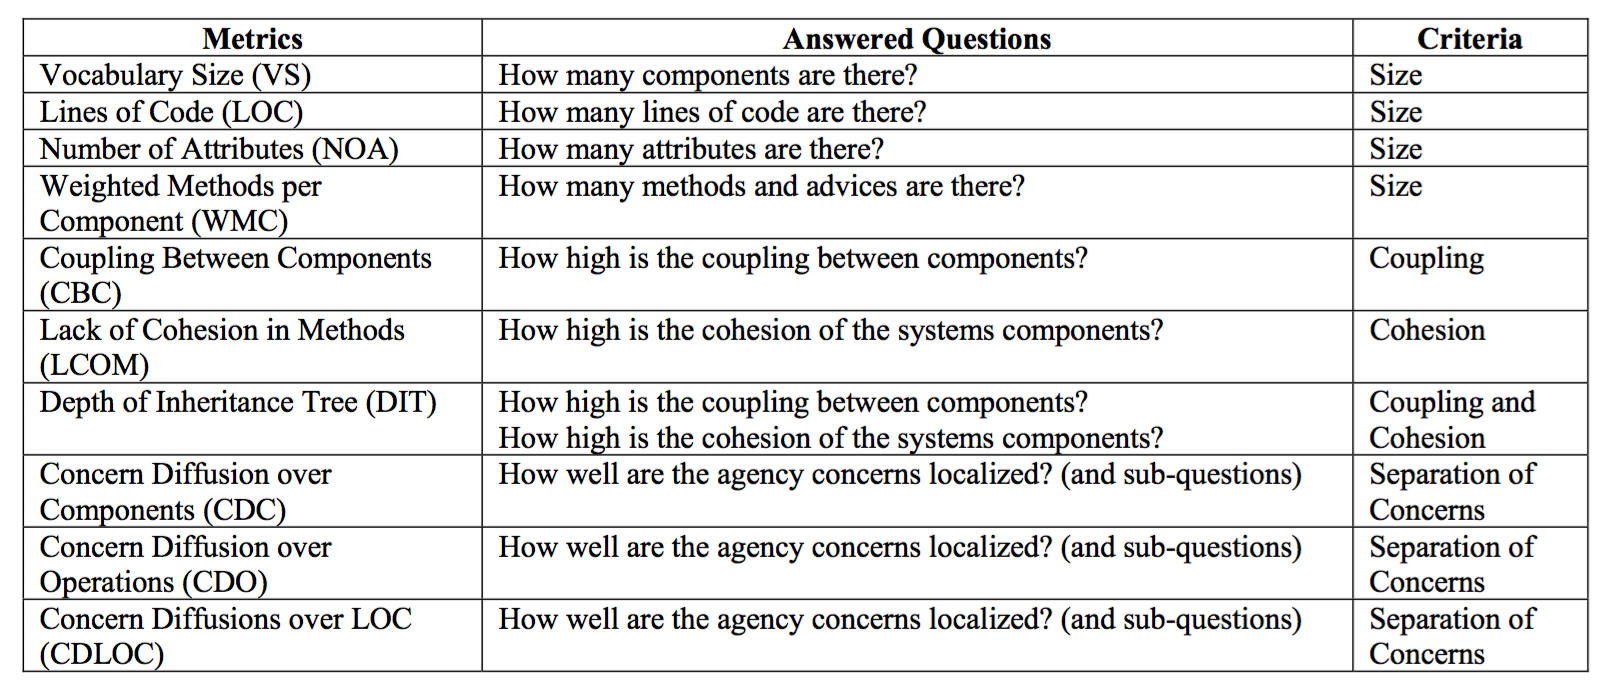
\includegraphics[width=.9\textwidth]{figures/metrics_questions.png}
  	\caption{Metrics and Goal/Question/Metric approach \cite{garcia2003agents}}
  	\label{fig:metrics_questions}
\end{figure}

